\chapter{TMS-EEG and F-Tract comparison}\label{ch:compare}

This chapter is devoted to the following questions: If we use TMS-EEG instead of iEEG (used in F-Tract), does the response still correlate with structural connectivity and communication metrics?  What are the similarities and what are the discrepancies? 

\section{Comparison of the correlations}\label{sec:compare-correlations_F-Tract-TMS}

Figure \ref{fig:compare-correlations_F-Tract-TMS} shows together the correlation coefficients of response probability or other characteristics with structural connectivity and communication metrics for 200 ms responses. 

TMS-EEG correlations are lower than correlations for F-Tract, no matter how we characterize the response. That was expected because the TMS stimulation has to get through the skull and other tissues before it enters the target region, and also the EEG measurement is performed through the head and source-reconstructed afterward, which all adds noise to the data.

Looking at the communication metrics, both TMS-EEG and F-Tract correlate best with the shortest path efficiency. An interesting observation is that if the response is characterized by first peak height, it correlates better with shortest path efficiency calculated using structural connectivity weights than lengths.

Another interesting question is how much can be explained by the Euclidean distance of the regions. As discussed in Chapter \ref{ch:ftract}, there are significant partial correlations for F-Tract probabilities and amplitudes even when Euclidean distance is controlled. We can also see in Figure \ref{fig:compare-correlations_F-Tract-TMS} that some of the communication metrics achieve higher correlations with response probability than the Euclidean distance for F-Tract. None of this is true for the TMS-EEG data. There are no significant partial correlations and the correlations of responses with communication metrics are lower than with Euclidean distance.\footnote{It is like that also for the other TMS-EEG thresholds and response lengths discussed in Chapter \ref{ch:pytepfit}.} 

This means that even though we might get some insight by studying the TMS-EEG from the perspective of communication metrics, we should keep in mind that various aspects of the response (AUC, the first peak height) are largely driven by the Euclidean distance. 

\begin{figure}
  \begin{center}
    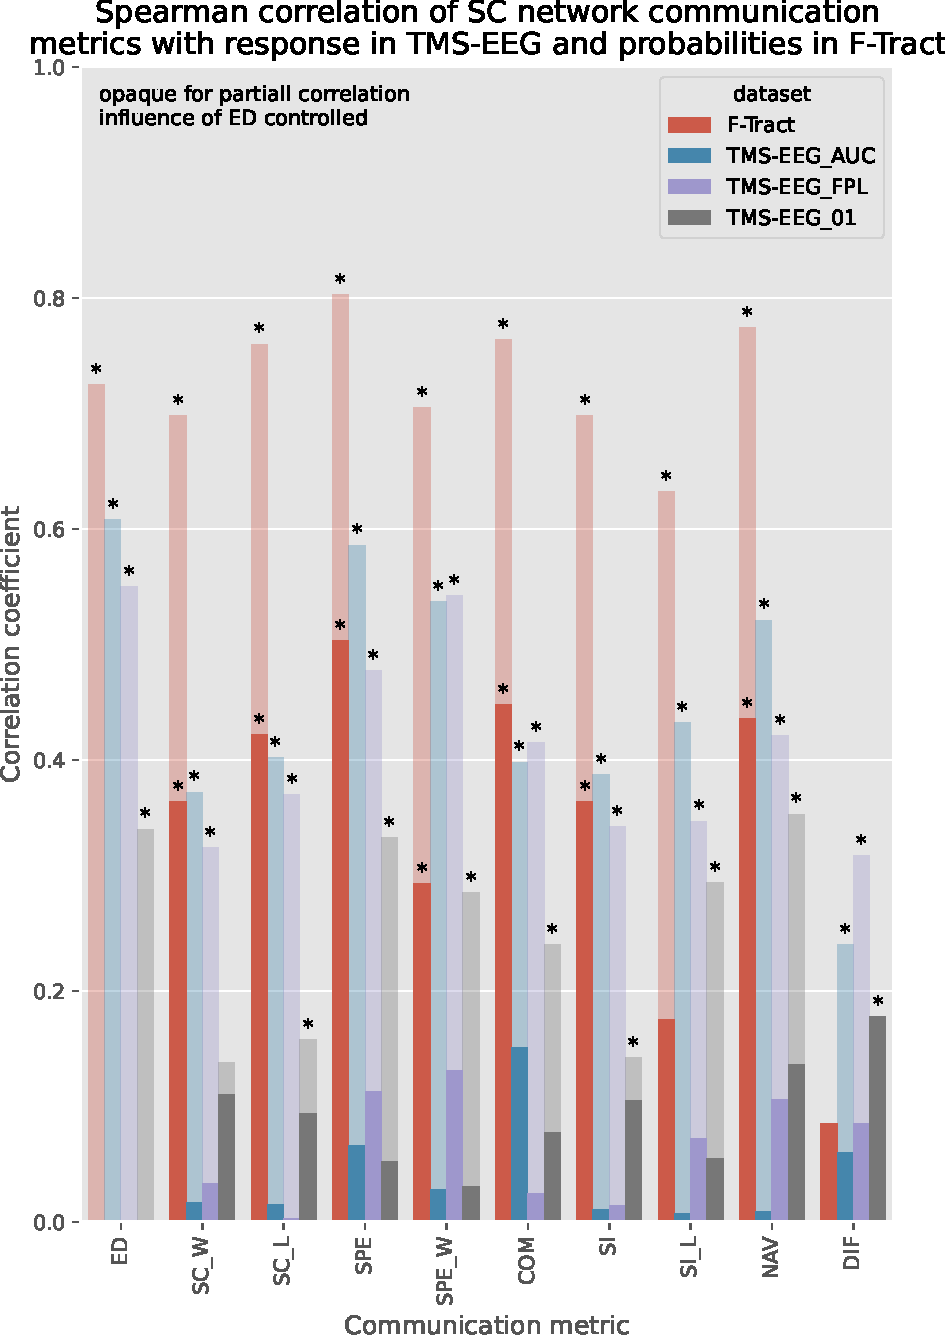
\includegraphics[width=0.89\textwidth]{images/nootebook_generated/tmseeg_ftract_comparison_results/200ms/Spearman_correlation_of_SC_network_communication_metrics_with_response_in_TMS-EEG_and_probabilities_in_F-Tract.pdf}
  \end{center}
  \caption[Comparison of correlations for F-Tract and TMS-EEG]{Comparison of correlations (absolute value) of response probability in F-Tract and TMS-EEG response characterized binary (01), by AUC and by the first peak latency (FPT) and structural connectivity and derived communication metrics. Asterisks denote a significant correlation ($p<0.05$). All the responses 200 ms long, structural connectivity based on Mica-Mics dataset with Rosen and Halgren's preprocessing. Threshold 8 in $z$-scored TMS-EEG.}
  \label{fig:compare-correlations_F-Tract-TMS}
\end{figure}

\section{Parcellations mapping}\label{sec:dice}

Direct comparison of the TMS-EEG and F-Tract results is not possible, because they do not share the same brain parcellation. The TMS-EEG dataset is published in Schaefer200 parcellation, which is not available for F-Tract. Because of that, it is necessary to find a mapping between Glasser and Schaefer200 parcellation.

Lawrence et al. published a paper \textit{Standardizing human brain parcellations} \cite{lawrence_standardizing_2021} discussing the issue of mapping between distinct brain parcellations. They propose the Dice coefficient \cite{dice_measures_1945} as a possibility of similarity evaluation between ROIs across parcellations. 

For two ROIs $A$ and $B$, each consisting of a set of voxels, the Dice coefficient of association is calculated as  
$$
\frac{2 \cdot |A\cap B|}{|A|+|B|}.
$$
the score is a ratio of the overlap of the regions to the sum of their sizes. It is higher for regions with a big overlap with respect to their sizes.

Lawrence et al. provide a function for calculations of Dice scores between parcellations in Neuroparc repository at GitHub.\footnote{\url{https://github.com/neurodata/neuroparc/blob/5a5e7469671e65cb58087c47b69d0edb71dc2966/scripts/dice_correlation.py}} Using that, Dice score map between Schaefer200 and Glasser parcellations was created.

Having the matrix with Dice scores for each pair of ROIs from Schaefer200 and Glasser, the easiest way to get comparable results is to assign one Schaefer200 ROI to each Glasser ROI based one the highest Dice coefficient (or vice versa, assign Glasser to Schaefer200 ROI). We can use this as a mapping for the vector of response probabilities in F-Tract and response AUC or other characteristics in TMS-EEG. 

\subsection{Stimulated site}\label{sec:parcellations-mapping-stimulated_roi}

Diving into the mapping of the parcellations, we found a discrepancy in the TMS-EEG data. The data-describing paper by Biabani et al. \cite{biabani_characterizing_2019} declares they stimulated the primary motor cortex, which is denoted \texttt{4\_L} in Glasser parcellation. Using the Dice mapping, this region has the highest overlap with ROI \texttt{7Networks\_LH\_SomMot\_15} in Schaefer200 parcellation. 

However, the source-reconstruction of the TMS-EEG data by Momi et al. \cite{momi_tms-evoked_2023} contains a vector indicating the stimulation weights for ROIs in Schaefer200. According to that, the stimulation target was \texttt{7Networks\_LH\_SomMot\_9} and \texttt{7Networks\_LH\_SomMot\_10} was affected a bit. Using the Dice scores again, ROI \texttt{7Networks\_LH\_SomMot\_9} has the biggest overlap with ROI \texttt{1\_L} in Glasser parcellation, followed by \texttt{3b\_L}. It has no overlap with ROI \texttt{4\_L}.

Because we use the TMS-EEG data in Schaefer200 parcellation, we decided to use \texttt{3b\_L} as a corresponding stimulation site in Glasser for the analysis, even though it is not the primary motor cortex. We chose \texttt{3b\_L} instead of \texttt{1\_L} because they are close to each other, both have an overlap with \texttt{7Networks\_LH\_SomMot\_9} and there are much more data in F-Tract for \texttt{3b\_L} stimulation than for \texttt{1\_L} stimulation, which is better for the analysis. 

\subsection{Comparison of F-Tract and TMS-EEG responses}

Section \ref{sec:compare-correlations_F-Tract-TMS} discusses that there are similarities in correlations between the stimulus responses in F-Tract and TMS-EEG and communication metrics. Now, let us see the relationship between responses in F-Tract and TMS-EEG. Are the responses structurally similar? If the same site is stimulated, does the strength of activation in TMS-EEG correspond to the response probability in F-Tract?

There is a significant correlation between AUC in TMS-EEG and response probability (Spearman correlation coefficient is $r=0.60$). If we look at the first peak height instead of AUC, there is again a significant correlation with the probability (Spearman correlation coefficient $r=-0.56$). The correlation is negative -- the responses with higher probabilities occur faster. 

Figure \ref{fig:response_tmsAUC-ftract_scatter} shows the response probability in F-Tract vs AUC in TMS-EEG. We see that there are regions in the somatomotor area that have a high probability of activation but the value of AUC is not exceptionally high and, on the contrary, regions in the salience/ventral attention area that do not have that high probability of activation according to F-Tract, but very high AUC. Figure \ref{fig:response_tmsFP-ftract_scatter} shows the comparison for the first peak latency instead of AUC. 

\begin{figure}
  \begin{center}
    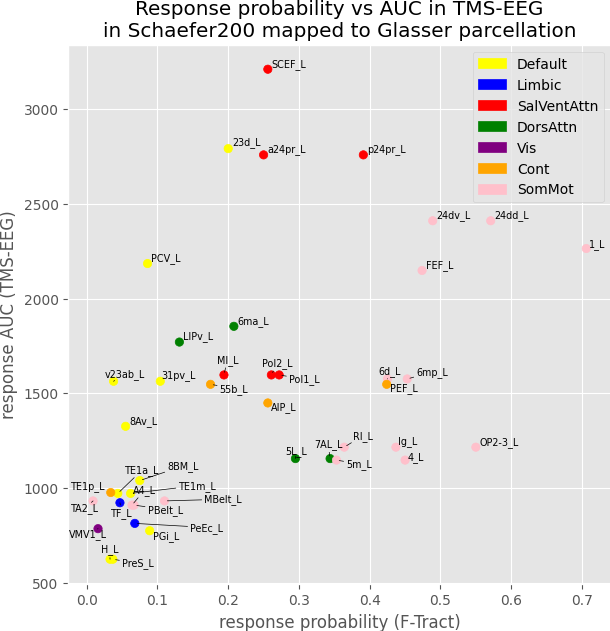
\includegraphics[width=\textwidth]{images/nootebook_generated/tmseeg_ftract_responses_comparison/AUC/Response_probability_vs_AUC_in_TMS-EEG_in_Schaefer200_mapped_to_Glasser_parcellation.png}
  \end{center}
  \caption[F-Tract probabilities vs TMS-EEG AUC]{F-Tract probabilities vs TMS-EEG AUC for 200 ms response length and threshold 8 in TMS-EEG. ROIs labeled based on Glasser parcellation and colored based on Yeo7 network extracted from Schaefer200 parcellation, plotted if the response value not \texttt{nan} in both F-Tract and AUC. Each Glasser ROI was assigned to Schaefer200 ROI based on the highest Dice score.}
  \label{fig:response_tmsAUC-ftract_scatter}
\end{figure}

\begin{figure}
  \begin{center}
    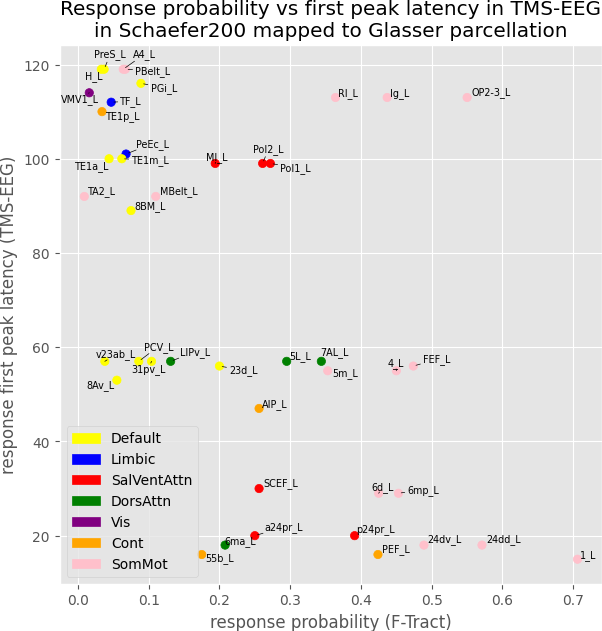
\includegraphics[width=\textwidth]{images/nootebook_generated/tmseeg_ftract_responses_comparison/FP/Response_probability_vs_first_peak_latency_in_TMS-EEG_in_Schaefer200_mapped_to_Glasser_parcellation.png}
  \end{center}
  \caption[F-Tract probabilities vs TMS-EEG first peak latency]{F-Tract probabilities vs TMS-EEG first peak latency for 200 ms response length and threshold 8 in TMS-EEG. ROIs labeled based on Glasser parcellation and colored based on Yeo7 network extracted from Schaefer200 parcellation, plotted if the response value not \texttt{nan} in both F-Tract and AUC. Each Glasser ROI was assigned to Schaefer200 ROI based on the highest Dice score.}
  \label{response_tmsFP-ftract_scatter}
\end{figure}